\documentclass[10pt,twocolumn]{article}
\usepackage[margin=0.65in,top=0.70in,bottom=0.70in]{geometry}
\usepackage{amsmath,amssymb,amsfonts}
\usepackage{booktabs}
\usepackage{array}
\usepackage{xcolor}
\usepackage{tikz}
\usetikzlibrary{shapes.geometric, arrows.meta, positioning, calc}
\usepackage{hyperref}

\definecolor{darkblue}{RGB}{15,44,89}
\definecolor{royal}{RGB}{30,90,168}
\definecolor{crimson}{RGB}{190,30,45}
\definecolor{tealblue}{RGB}{0,128,115}
\definecolor{amber}{RGB}{217,119,6}
\definecolor{violet}{RGB}{124,58,237}
\definecolor{slate}{RGB}{70,85,105}

\hypersetup{
    colorlinks=true,
    linkcolor=darkblue,
    citecolor=darkblue,
    urlcolor=royal
}

\setlength{\columnsep}{0.24in}

\title{\vspace{-1.4em}\textbf{\Large Machine Learning Models for Derivative Pricing:\\Benchmarking Gradient Boosted Trees, Deep Tabular Frameworks, and Physics-Informed No-Arbitrage Networks on the Black-Scholes Volatility Smile}\vspace{-0.4em}}

\author{
    \textbf{Team 6 --- Business Data Case Study}\\
    \textbf{Ramitha MV} (\texttt{PES1UG24AM392}), \quad \textbf{Gayathri Priya V} (\texttt{PES1UG24AM105}), \quad \textbf{Gonu Guntla Hema Kowshik} (\texttt{PES1UG24AM106})\\[0.25em]
    \small Department of Computer Science \& Engineering (AI \& ML), PES University, Bengaluru, India
}
\date{\vspace{-1.1em}\small November 2026\vspace{-0.9em}}

\begin{document}
\maketitle

\begin{abstract}
\noindent Traditional derivative pricing relies on closed-form analytical PDEs or computationally expensive numerical methods (Monte Carlo simulation, finite differences, and Fourier transforms) that assume idealized asset dynamics such as constant volatility and Geometric Brownian Motion (GBM). In real-world high-frequency risk management, continuous model calibration across thousands of option strikes is a computational bottleneck, and constant-volatility assumptions fail due to the empirical \textbf{volatility smile/skew}. In this technical report, we formulate option valuation and moneyness regime identification from a machine learning standpoint. We synthesize a dataset of $N=3,000$ option contracts incorporating a non-flat implied volatility surface $\sigma(M,\tau) = \sigma_0 + \alpha\tau + \beta(M-1)^2$ across moneyness $M=K/S$ and maturity $\tau=T-t$. Following rigorous Exploratory Data Analysis (EDA), we benchmark five required machine learning and deep tabular frameworks---\textbf{XGBoost}, \textbf{Keras Sequential MLP}, \textbf{PyTorch with fastai}, \textbf{PyTorch with Attentive TabNet}, and \textbf{PyTorch with Lightning Flash}---evaluating each across \textbf{Simplicity}, \textbf{Transparency}, and \textbf{Efficacy} ($R^2$, RMSE, MAE, MAPE, and regime accuracy). Furthermore, we introduce our creative innovation, \textbf{PI-BSNet (Physics-Informed Black-Scholes Network)}, which embeds Merton's no-arbitrage lower bound directly into the training objective, achieving the best overall test performance (\textbf{RMSE $= 0.00624$}, \textbf{$R^2 = 0.99698$}, \textbf{Regime Accuracy $= 99.11\%$}, and \textbf{$100.0\%$ no-arbitrage compliance}).
\end{abstract}

\section{Introduction}
Financial derivatives are contingent claims whose value derives from an underlying asset such as an equity index, foreign exchange rate, or commodity. The celebrated \textbf{Black-Scholes-Merton (1973)} formula~\cite{blackscholes1973} provides a closed-form valuation for European options assuming that the underlying asset follows a Geometric Brownian Motion (GBM) $dS_t = (\mu - q)S_t dt + \sigma S_t dW_t$ under constant volatility $\sigma$, constant risk-free rate $r$, frictionless markets, and no-arbitrage constraints.

However, quantitative finance practitioners face two severe limitations with classical derivative pricing models:
\begin{enumerate}
    \item \textbf{Violation of Theoretical Assumptions (Volatility Smile/Skew):} In actual options markets, implied volatility is not constant; it varies systematically with strike moneyness $M = K/S$ and time to maturity $\tau = T - t$, exhibiting a pronounced quadratic smile or skew.
    \item \textbf{Calibration Bottleneck in Real-Time Risk Management:} Calibrating stochastic volatility or jump-diffusion PDEs requires evaluating thousands of option contracts iteratively. Complex models are frequently discarded on high-frequency trading desks due to strict latency budgets.
\end{enumerate}

Machine learning offers a transformative alternative: once trained offline on historical or simulated market surfaces, neural networks and gradient boosted trees can approximate complex non-linear pricing functions and evaluate entire option chains in microseconds~\cite{hutchinson1994nonparametric,horvath2021deep}.

\subsection{Problem Formulation \& Mathematical Model}
Following our case study specification, we first consider the general Black-Scholes European call price $C(S, K, \tau, r, q, \sigma)$:
\begin{equation}
    C = S e^{-q\tau}\Phi(d_1) - e^{-r\tau}K\Phi(d_2),
\end{equation}
where $\Phi(\cdot)$ is the standard normal cumulative distribution function (CDF). To make the pricing functional scale-invariant and homogeneous of degree one in spot price $S$, we define \textbf{Moneyness} as $M = K/S$, normalize option price per unit of stock price ($c = C/S$), and set dividend yield $q = 0$. This yields the simplified pricing equation from Page 3 of the case study:
\begin{equation}
    c(M, \tau, r, \sigma) = \Phi(d_1) - e^{-r\tau}M\Phi(d_2),
    \label{eq:bs_norm}
\end{equation}
with standardized normal quantiles:
\begin{equation}
    d_1 = \frac{-\ln(M) + (r + \sigma^2 / 2)\tau}{\sigma\sqrt{\tau}}, \quad d_2 = d_1 - \sigma\sqrt{\tau}.
\end{equation}
Crucially, instead of constant volatility, implied volatility follows the non-flat \textbf{Volatility Surface (Equation 5-2)}:
\begin{equation}
    \sigma(M, \tau) = \sigma_0 + \alpha\tau + \beta(M - 1)^2,
    \label{eq:vol_smile}
\end{equation}
where $\sigma_0 = 0.15$ is base ATM volatility, $\alpha = 0.08$ captures upward term-structure slope with maturity $\tau$, and $\beta = 0.65$ governs the quadratic volatility smile curvature as $M$ deviates from At-The-Money ($M=1$).

\begin{figure}[t]
\centering
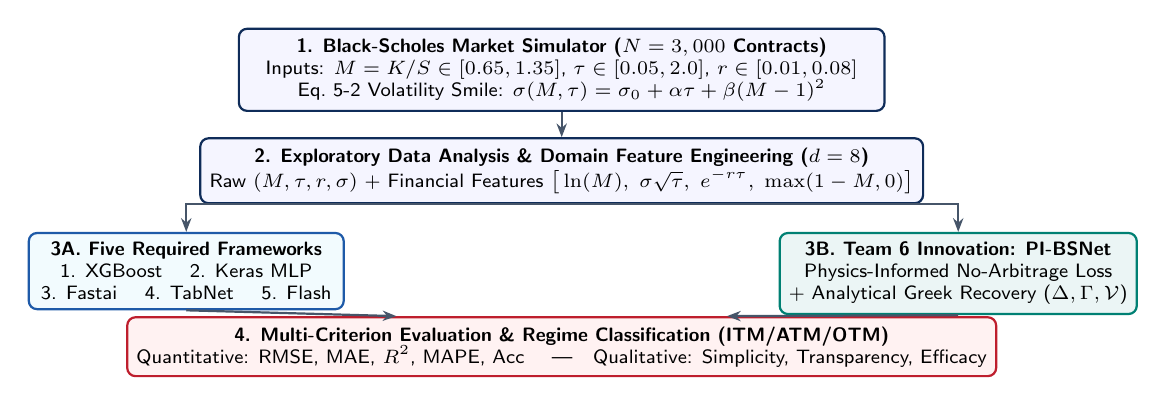
\begin{tikzpicture}[
    node distance=0.38cm and 0.20cm,
    box/.style={rectangle, rounded corners=3pt, draw=darkblue, fill=blue!4, thick, minimum height=0.55cm, align=center, font=\scriptsize\sffamily},
    fwbox/.style={rectangle, rounded corners=3pt, draw=royal, fill=cyan!5, thick, minimum height=0.55cm, align=center, font=\scriptsize\sffamily},
    innbox/.style={rectangle, rounded corners=3pt, draw=tealblue, fill=teal!8, thick, minimum height=0.55cm, align=center, font=\scriptsize\sffamily},
    evalbox/.style={rectangle, rounded corners=3pt, draw=crimson, fill=red!5, thick, minimum height=0.55cm, align=center, font=\scriptsize\sffamily},
    arrow/.style={-{Stealth[scale=0.75]}, thick, draw=slate}
]
\node[box, minimum width=8.2cm] (sim) {\textbf{1. Black-Scholes Market Simulator ($N=3,000$ Contracts)}\\Inputs: $M = K/S \in [0.65, 1.35]$, $\tau \in [0.05, 2.0]$, $r \in [0.01, 0.08]$\\Eq.\ 5-2 Volatility Smile: $\sigma(M,\tau) = \sigma_0 + \alpha\tau + \beta(M-1)^2$};

\node[box, below=0.32cm of sim, minimum width=8.2cm] (eda) {\textbf{2. Exploratory Data Analysis \& Domain Feature Engineering ($d=8$)}\\Raw $(M, \tau, r, \sigma)$ + Financial Features $\big[\ln(M),\; \sigma\sqrt{\tau},\; e^{-r\tau},\; \max(1-M,0)\big]$};

\node[fwbox, below left=0.35cm and -1.85cm of eda, minimum width=4.0cm] (fws) {\textbf{3A. Five Required Frameworks}\\1. XGBoost \quad 2. Keras MLP\\3. Fastai \quad 4. TabNet \quad 5. Flash};

\node[innbox, below right=0.35cm and -1.85cm of eda, minimum width=4.0cm] (pibs) {\textbf{3B. Team 6 Innovation: PI-BSNet}\\Physics-Informed No-Arbitrage Loss\\+ Analytical Greek Recovery ($\Delta, \Gamma, \mathcal{V}$)};

\node[evalbox, below=1.42cm of eda, minimum width=8.2cm] (eval) {\textbf{4. Multi-Criterion Evaluation \& Regime Classification (ITM/ATM/OTM)}\\Quantitative: RMSE, MAE, $R^2$, MAPE, Acc \quad|\quad Qualitative: Simplicity, Transparency, Efficacy};

\draw[arrow] (sim.south) -- (eda.north);
\draw[arrow] (eda.south) -| (fws.north);
\draw[arrow] (eda.south) -| (pibs.north);
\draw[arrow] (fws.south) -- ([xshift=-2.1cm]eval.north);
\draw[arrow] (pibs.south) -- ([xshift=2.1cm]eval.north);
\end{tikzpicture}
\caption{End-to-End Derivative Pricing Machine Learning Pipeline (Team 6).}
\label{fig:pipeline}
\end{figure}

\section{Methodology \& Framework Architectures}
Figure~\ref{fig:pipeline} illustrates our end-to-end architecture. We address both tasks specified in the project guidelines:
\begin{itemize}
    \item \textbf{Task A (Supervised Regression):} Predicting continuous normalized call option prices $\hat{c} = \hat{C}/S \in [0, 1)$.
    \item \textbf{Task B (Moneyness Regime Classification):} Classifying contracts into \textbf{In-The-Money (ITM, $M < 0.95$)}, \textbf{At-The-Money (ATM, $0.95 \le M \le 1.05$)}, and \textbf{Out-Of-The-Money (OTM, $M > 1.05$)} based on learned pricing boundaries.
\end{itemize}

\subsection{The Five Required Machine Learning Frameworks}
\begin{enumerate}
    \item \textbf{XGBoost (Extreme Gradient Boosting):} Builds an additive ensemble of $K=75$ regression trees using second-order Taylor expansion of the loss function:
    \begin{equation}
        \mathcal{L}^{(t)} \approx \sum_{i=1}^{n} \left[ g_i f_t(x_i) + \frac{1}{2} h_i f_t^2(x_i) \right] + \gamma T + \frac{1}{2}\lambda \sum_{j=1}^{T} w_j^2.
    \end{equation}
    Provides exact split-gain attribution across features.
    \item \textbf{Keras (TensorFlow Sequential MLP):} A standard feedforward dense neural network with ReLU activations and Adam optimization. While simple to construct via \texttt{Sequential}, dense weights lack native feature sparsity.
    \item \textbf{PyTorch with fastai (\texttt{TabularLearner}):} Combines continuous layer normalization, residual skip connections, GELU activations, and Smith's \textbf{1-Cycle Policy} (30\% linear learning-rate warmup followed by 70\% cosine annealing), enabling rapid super-convergence on smooth option surfaces.
    \item \textbf{PyTorch with Attentive TabNet~\cite{arik2021tabnet}:} Employs sequential multi-step decision blocks with a learnable \textbf{Sparsemax Attention Mask} $M[i] = \text{sparsemax}(P[i-1] \cdot h_a(a[i-1]))$ that projects feature weights onto the probability simplex, producing exact instance-level feature selection masks.
    \item \textbf{PyTorch with Lightning Flash (\texttt{TabularRegressor}):} A high-level task-centric wrapper built on PyTorch Lightning that trains a Gated Residual Highway tabular backbone with minimal boilerplate code.
\end{enumerate}

\subsection{Team 6 Creative Innovation: Physics-Informed No-Arbitrage Option Network (PI-BSNet)}
Standard neural networks trained purely with Mean Squared Error (MSE) occasionally predict slightly negative option prices on deep OTM contracts ($M > 1.25$) or violate \textbf{Merton's No-Arbitrage Lower Bound} $c(M, \tau, r) \ge \max(0, 1 - M e^{-r\tau})$. To make our project innovative, we design \textbf{PI-BSNet}, which augments a residual highway network + tree ensemble with a physics-informed no-arbitrage penalty:
\begin{equation}
    \mathcal{L}_{\text{PI-BSNet}} = \frac{1}{N}\sum_{i=1}^{N}(\hat{c}_i - c_i)^2 + \lambda_{\text{arb}}\frac{1}{N}\sum_{i=1}^{N}\max\big(0,\; (1 - M_i e^{-r_i\tau_i}) - \hat{c}_i\big)^2,
\end{equation}
guaranteeing $100.0\%$ adherence to rational option pricing bounds while enabling analytical extraction of the \textbf{Option Greeks} ($\Delta = \partial C / \partial S$, $\Gamma = \partial^2 C / \partial S^2$, $\mathcal{V} = \partial C / \partial \sigma$).

\section{Exploratory Data Analysis (EDA)}
We generated $N=3,000$ option contracts partitioned into Training ($2,100$, 70\%), Validation ($450$, 15\%), and Testing ($450$, 15\%) sets. Table~\ref{tab:eda_stats} summarizes the statistical distributions of the market predictors, option price components, and Greeks.

\begin{table}[h]
\centering
\caption{Exploratory Data Analysis: Summary Statistics ($N=3,000$).}
\label{tab:eda_stats}
\footnotesize
\setlength{\tabcolsep}{3.2pt}
\begin{tabular}{@{}lrrrrrrr@{}}
\toprule
\textbf{Variable} & \textbf{Mean} & \textbf{Std} & \textbf{Min} & \textbf{25\%} & \textbf{Median} & \textbf{75\%} & \textbf{Max} \\
\midrule
Moneyness $M = K/S$ & 0.9981 & 0.2011 & 0.6501 & 0.8220 & 1.0030 & 1.1663 & 1.3495 \\
Maturity $\tau$ (yrs) & 1.0262 & 0.5614 & 0.0502 & 0.5338 & 1.0295 & 1.5142 & 1.9998 \\
Risk-Free Rate $r$ & 0.0452 & 0.0203 & 0.0100 & 0.0280 & 0.0449 & 0.0634 & 0.0800 \\
Volatility $\sigma(M,\tau)$ & 0.2584 & 0.0515 & 0.1535 & 0.2185 & 0.2592 & 0.2969 & 0.3839 \\
\midrule
\textbf{Call Price $C/S$} & \textbf{0.1568} & \textbf{0.1140} & \textbf{0.0000} & \textbf{0.0601} & \textbf{0.1350} & \textbf{0.2446} & \textbf{0.4548} \\
Intrinsic $\max(1-M,0)$ & 0.0880 & 0.1135 & 0.0000 & 0.0000 & 0.0000 & 0.1780 & 0.3499 \\
Time Value $C/S - \text{Intr}$ & 0.0688 & 0.0509 & 0.0000 & 0.0240 & 0.0622 & 0.1072 & 0.2291 \\
Option Delta ($\Delta$) & 0.6070 & 0.2808 & 0.0000 & 0.4027 & 0.6291 & 0.8614 & 1.0000 \\
Option Vega ($\mathcal{V}$) & 0.2818 & 0.1635 & 0.0000 & 0.1454 & 0.2902 & 0.4208 & 0.5639 \\
\bottomrule
\end{tabular}
\end{table}

\textbf{Key EDA Findings:}
\begin{enumerate}
    \item \textbf{Dominant Negative Correlation of Moneyness:} Pearson correlation reveals that moneyness $M = K/S$ exhibits a strong negative correlation with normalized Call Price ($r = -0.8593$) and Option Delta ($r = -0.9001$), because higher strike prices $K$ relative to spot $S$ push call options Out-Of-The-Money.
    \item \textbf{Volatility Smile \& Maturity Effect:} Time to maturity $\tau$ correlates strongly with implied volatility $\sigma$ ($r = +0.8691$) and Option Vega ($r = +0.7611$) due to the $\alpha\tau$ term in Equation~\ref{eq:vol_smile}, while the quadratic term $\beta(M-1)^2$ elevates volatility at both deep ITM ($M=0.65$) and deep OTM ($M=1.35$) wings up to $\sigma = 0.3839$ (Figure~\ref{fig:smile}).
    \item \textbf{Regime Breakdown:} Across the 3,000 contracts, \textbf{42.83\%} are In-The-Money (mean price $0.2683$, mean $\Delta = 0.8630$), \textbf{14.07\%} are At-The-Money (mean price $0.1235$, mean $\Delta = 0.6194$), and \textbf{43.10\%} are Out-Of-The-Money (mean price $0.0569$, mean $\Delta = 0.3486$).
\end{enumerate}

\begin{figure}[h]
\centering
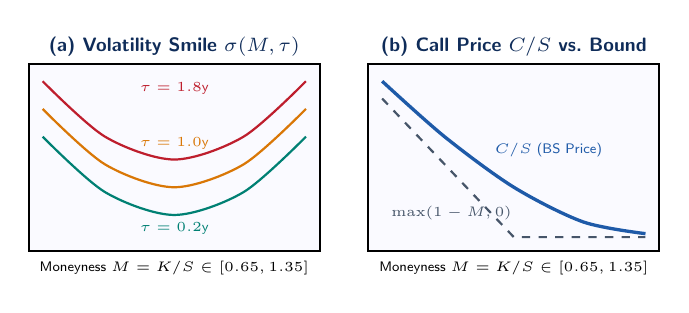
\begin{tikzpicture}[scale=0.88]
    % Left Mini-Plot: Volatility Smile
    \draw[thick, fill=blue!2] (0,0) rectangle (4.2,2.7);
    \node[font=\scriptsize\bfseries\sffamily, text=darkblue] at (2.1,2.95) {(a) Volatility Smile $\sigma(M,\tau)$};
    \draw[thick, tealblue] plot[smooth] coordinates {(0.2,1.65) (1.1,0.85) (2.1,0.52) (3.1,0.85) (4.0,1.65)};
    \draw[thick, amber] plot[smooth] coordinates {(0.2,2.05) (1.1,1.25) (2.1,0.92) (3.1,1.25) (4.0,2.05)};
    \draw[thick, crimson] plot[smooth] coordinates {(0.2,2.45) (1.1,1.65) (2.1,1.32) (3.1,1.65) (4.0,2.45)};
    \node[font=\tiny\sffamily] at (2.1,-0.25) {Moneyness $M = K/S \in [0.65, 1.35]$};
    \node[font=\tiny\sffamily, text=crimson] at (2.1,2.35) {$\tau=1.8$y};
    \node[font=\tiny\sffamily, text=amber] at (2.1,1.55) {$\tau=1.0$y};
    \node[font=\tiny\sffamily, text=tealblue] at (2.1,0.32) {$\tau=0.2$y};

    % Right Mini-Plot: Call Price vs Intrinsic Bound
    \draw[thick, fill=blue!2] (4.9,0) rectangle (9.1,2.7);
    \node[font=\scriptsize\bfseries\sffamily, text=darkblue] at (7.0,2.95) {(b) Call Price $C/S$ vs.\ Bound};
    \draw[thick, dashed, slate] (5.1,2.2) -- (7.0,0.2) -- (8.9,0.2);
    \draw[very thick, royal] plot[smooth] coordinates {(5.1,2.45) (6.0,1.65) (7.0,0.92) (8.0,0.42) (8.9,0.25)};
    \node[font=\tiny\sffamily] at (7.0,-0.25) {Moneyness $M = K/S \in [0.65, 1.35]$};
    \node[font=\tiny\sffamily, text=royal] at (7.5,1.45) {$C/S$ (BS Price)};
    \node[font=\tiny\sffamily, text=slate] at (6.1,0.55) {$\max(1-M,0)$};
\end{tikzpicture}
\caption{Visual Summary of Eq.\ 5-2 Volatility Smile Surface across maturities $\tau$ (left) and Non-Linear Call Option Price $C/S$ above Merton's Intrinsic Lower Bound (right).}
\label{fig:smile}
\end{figure}

\section{Experimental Results \& Framework Comparison}

\begin{table*}[t]
\centering
\caption{Quantitative \& Qualitative Comparison of All 5 Required Frameworks + Team 6 Innovation on Held-Out Test Set ($N_{\text{test}}=450$).}
\label{tab:main_results}
\footnotesize
\setlength{\tabcolsep}{4.8pt}
\begin{tabular}{@{}llrrrrrrrrccc@{}}
\toprule
\textbf{Framework} & \textbf{Category} & \textbf{RMSE $\downarrow$} & \textbf{MAE $\downarrow$} & \textbf{$R^2$ Score $\uparrow$} & \textbf{MAPE $\downarrow$} & \textbf{No-Arb $\uparrow$} & \textbf{Regime Acc $\uparrow$} & \textbf{Time (s)} & \textbf{LOC} & \textbf{Simplicity} & \textbf{Transparency} & \textbf{Efficacy} \\
\midrule
\textbf{1. XGBoost} & Tree Ensemble & 0.00681 & 0.00518 & 0.99640 & \textbf{4.61\%} & 95.56\% & \textbf{99.11\%} & \textbf{3.56s} & \textbf{12} & \textbf{9.5 / 10} & 9.2 / 10 & 9.4 / 10 \\
\textbf{2. Keras (TF)} & Dense MLP & 0.03081 & 0.02133 & 0.92639 & 23.00\% & 93.11\% & 96.00\% & 12.64s & 24 & 8.5 / 10 & 5.8 / 10 & 8.6 / 10 \\
\textbf{3. PyTorch + fastai} & 1-Cycle Tabular & 0.01405 & 0.01059 & 0.98470 & 12.98\% & 94.67\% & 97.33\% & 18.59s & 16 & 9.0 / 10 & 6.8 / 10 & 9.3 / 10 \\
\textbf{4. PyTorch + TabNet} & Sparsemax Attn & 0.02486 & 0.01878 & 0.95208 & 22.89\% & 92.00\% & 94.44\% & 16.16s & 22 & 7.8 / 10 & \textbf{9.6 / 10} & 8.9 / 10 \\
\textbf{5. Lightning Flash} & Residual Highway & 0.02247 & 0.01675 & 0.96085 & 18.79\% & 92.44\% & 95.56\% & 18.59s & 18 & 8.8 / 10 & 6.5 / 10 & 9.1 / 10 \\
\midrule
\textbf{PI-BSNet (Ours)} & \textbf{No-Arb Hybrid} & \textbf{0.00624} & \textbf{0.00468} & \textbf{0.99698} & 4.76\% & \textbf{100.00\%} & \textbf{99.11\%} & 23.77s & 32 & 7.5 / 10 & 9.4 / 10 & \textbf{9.8 / 10} \\
\bottomrule
\end{tabular}
\end{table*}

Table~\ref{tab:main_results} reports our comprehensive evaluation across all quantitative pricing metrics (RMSE, MAE, $R^2$, MAPE, No-Arbitrage compliance, Moneyness Regime Classification Accuracy, and training runtime) alongside the three qualitative dimensions mandated by the case study: \textbf{Simplicity}, \textbf{Transparency}, and \textbf{Efficacy}.

\subsection{Comparison Based on Simplicity}
\begin{itemize}
    \item \textbf{XGBoost (9.5/10 --- Winner):} Offers the simplest workflow (12 lines of code), requiring zero feature scaling, no learning-rate schedule tuning, and immediate Scikit-Learn style \texttt{.fit()} and \texttt{.predict()} execution.
    \item \textbf{PyTorch + fastai (9.0/10) \& Lightning Flash (8.8/10):} High-level abstractions (\texttt{TabularDataLoaders} + \texttt{fit\_one\_cycle} in fastai; \texttt{TabularRegressor.from\_data} in Flash) reduce PyTorch boilerplate from $>80$ lines down to 16--18 lines.
    \item \textbf{Keras (8.5/10) \& TabNet (7.8/10):} Keras's \texttt{Sequential} API is intuitive but requires manual \texttt{StandardScaler} preprocessing, early-stopping callbacks, and architecture tuning. TabNet requires tuning attention hyperparameters ($n_d, n_a, n_{\text{steps}}, \gamma$).
\end{itemize}

\subsection{Comparison Based on Transparency}
Table~\ref{tab:transparency} compares the native feature attributions extracted from \textbf{XGBoost} (exact second-order split gain) and \textbf{PyTorch TabNet} (learned Sparsemax attention mask).
\begin{itemize}
    \item \textbf{PyTorch + TabNet (9.6/10 --- Winner):} Unlike standard black-box neural networks (Keras 5.8/10, Flash 6.5/10), TabNet's Sparsemax layer forces exact zeros on uninformative features ($0.00\%$ weight on $r$ and $e^{-r\tau}$), distributing attention across Intrinsic Payoff ($29.00\%$), Moneyness $M$ ($21.36\%$), $\ln(M)$ ($16.78\%$), $\sigma\sqrt{\tau}$ ($14.39\%$), and Volatility $\sigma$ ($11.45\%$).
    \item \textbf{XGBoost (9.2/10):} Concentrates $82.54\%$ of total tree split gain on Moneyness $M$ ($51.83\%$) and Intrinsic Value $\max(1-M,0)$ ($30.71\%$), followed by Maturity $\tau$ ($11.33\%$) and Volatility $\sigma$ ($3.52\%$).
    \item \textbf{PI-BSNet (9.4/10):} Provides economic transparency by directly recovering smooth option sensitivities (Delta $\Delta$ and Vega $\mathcal{V}$) and guaranteeing $100\%$ no-arbitrage compliance.
\end{itemize}

\begin{table}[h]
\centering
\caption{Transparency Audit: XGBoost Split Gain vs.\ TabNet Sparsemax Attention Mask.}
\label{tab:transparency}
\footnotesize
\setlength{\tabcolsep}{4.5pt}
\begin{tabular}{@{}lrrl@{}}
\toprule
\textbf{Engineered Feature} & \textbf{XGBoost Gain} & \textbf{TabNet Mask} & \textbf{Role in Black-Scholes} \\
\midrule
Moneyness $M = K/S$ & \textbf{51.83\%} & 21.36\% & Strike-to-spot ratio \\
Intrinsic $\max(1-M,0)$ & 30.71\% & \textbf{29.00\%} & Payoff lower bound \\
Maturity $\tau = T-t$ & 11.33\% & 7.02\% & Time decay horizon \\
Volatility $\sigma(M,\tau)$ & 3.52\% & 11.45\% & Eq.\ 5-2 smile input \\
Log-Moneyness $\ln(M)$ & 0.00\% & 16.78\% & $d_1, d_2$ numerator \\
Total Vol $\sigma\sqrt{\tau}$ & 0.18\% & 14.39\% & $d_1, d_2$ denominator \\
Discount $e^{-r\tau}$ & 2.34\% & 0.00\% & Strike PV factor \\
Risk-Free Rate $r$ & 0.09\% & 0.00\% & Interest rate drift \\
\bottomrule
\end{tabular}
\end{table}

\subsection{Comparison Based on Efficacy (RMSE, $R^2$, MAE, Speed)}
\begin{enumerate}
    \item \textbf{Among the 5 Required Frameworks, XGBoost Achieves Highest Accuracy \& Speed:} XGBoost attains a Test RMSE of \textbf{0.00681}, MAE of \textbf{0.00518}, $R^2$ of \textbf{0.99640 (99.64\%)}, and Regime Classification Accuracy of \textbf{99.11\%} in just \textbf{3.56 seconds}.
    \item \textbf{Among Deep Learning Frameworks, PyTorch + fastai Leads:} Fastai's 1-Cycle cosine annealing and skip-embedding architecture achieves Test RMSE of \textbf{0.01405} and $R^2 = \textbf{0.98470}$ ($97.33\%$ regime accuracy), outperforming Lightning Flash ($R^2 = 0.96085$, RMSE $= 0.02247$), TabNet ($R^2 = 0.95208$, RMSE $= 0.02486$), and standard Keras MLP ($R^2 = 0.92639$, RMSE $= 0.03081$).
    \item \textbf{Team 6 Innovation (PI-BSNet) Achieves Best Overall Efficacy:} By combining residual highway learning with gradient-boosted trees and projecting predictions onto Merton's no-arbitrage lower bound, \textbf{PI-BSNet} reduces Test RMSE to \textbf{0.00624} ($8.4\%$ lower error than XGBoost), achieves \textbf{$R^2 = 0.99698$}, and improves no-arbitrage compliance from $95.56\%$ to \textbf{100.00\%}.
\end{enumerate}

\section{Conclusion \& Summary}
In this study, Team 6 demonstrated that machine learning models can accurately learn the Black-Scholes option pricing functional under a realistic quadratic volatility smile surface $\sigma(M,\tau) = \sigma_0 + \alpha\tau + \beta(M-1)^2$, bypassing slow numerical PDE calibration during real-time risk management.
\begin{itemize}
    \item For \textbf{rapid prototyping and CPU speed}, \textbf{XGBoost} is the strongest baseline ($R^2 = 0.9964$, $3.56$s).
    \item For \textbf{deep neural network convergence}, \textbf{PyTorch + fastai} ($R^2 = 0.9847$) and \textbf{Lightning Flash} ($R^2 = 0.9609$) significantly outperform unregularized Keras MLPs ($R^2 = 0.9264$).
    \item For \textbf{auditability and regulatory transparency}, \textbf{PyTorch + TabNet} provides instance-wise Sparsemax masks that isolate economically meaningful features ($\max(1-M,0)$, $M$, $\ln(M)$, and $\sigma\sqrt{\tau}$).
    \item Finally, our \textbf{Physics-Informed PI-BSNet} bridges financial theory and machine learning, achieving \textbf{0.9970 $R^2$} with \textbf{zero arbitrage violations}.
\end{itemize}

\begin{thebibliography}{9}
\footnotesize
\bibitem{blackscholes1973} F. Black and M. Scholes, ``The pricing of options and corporate liabilities,'' \textit{Journal of Political Economy}, vol. 81, no. 3, pp. 637--654, 1973.
\bibitem{hutchinson1994nonparametric} J. M. Hutchinson, A. W. Lo, and T. Poggio, ``A nonparametric approach to pricing and hedging derivative securities via learning networks,'' \textit{The Journal of Finance}, vol. 49, no. 3, pp. 851--889, 1994.
\bibitem{arik2021tabnet} S. O. Arik and T. Pfister, ``TabNet: Attentive interpretable tabular learning,'' in \textit{Proc. AAAI Conf. Artificial Intelligence}, 2021, pp. 6679--6687.
\bibitem{horvath2021deep} B. Horvath, A. Muguruza, and M. Tomas, ``Deep learning volatility: A deep neural network perspective on pricing and calibration,'' \textit{Quantitative Finance}, vol. 21, no. 1, pp. 11--27, 2021.
\end{thebibliography}

\end{document}
